% ALMA-13B-R weight-only GPTQ: the precision grid, tables and figures.
%
%   python francesco/analysis/make_report.py   # regenerate tables.tex, detail.tex, figures.tex
%   pdflatex -output-directory=.. results.tex  # run this in francesco/results/tex/, twice
%
% tables.tex / detail.tex / figures.tex are generated -- edit make_report.py, not them.
% figures.tex \includegraphics from ../figures/, the .pdf written by make_report.py.
% To drop these into the paper instead, copy the preamble packages this file needs
% (booktabs, xcolor with the table option, graphicx) and \input the three chunks.
\documentclass[10pt]{article}
\usepackage[table]{xcolor}
\usepackage{booktabs}
\usepackage{graphicx}
\usepackage{caption}
\usepackage{geometry}
\geometry{margin=2.2cm}
\usepackage[hidelinks]{hyperref}

\captionsetup{font=small,labelfont=bf}

\title{ALMA-13B-R under weight-only GPTQ: 16 / 8 / 4 / 3 / 2 bits on WMT'22}
\author{}
\date{\today}

\begin{document}
\maketitle


\section*{What is in here}

ALMA-13B-R quantized by GPTQ (\texttt{GPTQModel} 4.2.5): weight-only, asymmetric,
group size 128, act-order, every Linear of the 40 decoder layers quantized, embeddings /
\texttt{lm\_head} / norms / scales left in fp16. Generation is beam 5, bf16, seed 42, the
protocol of \texttt{ours-beam} (the fp16 reproduction, which is the baseline here), scored
on WMT'22 for de, cs, zh, ru and WMT'21 for is. Table~\ref{tab:grid-avg} is the grid,
Table~\ref{tab:grid-delta} the cost against fp16, Table~\ref{tab:sizes} the checkpoint
sizes; per-direction numbers are in the appendix tables, and the raw
\texttt{outputs/baseline/<run>.tsv} files stay the machine-readable copy.

\section*{The grid}
\begin{table*}[t]
\centering
\footnotesize
\setlength{\tabcolsep}{4pt}
\begin{tabular}{lrrrrrrrrrr}
\toprule
& BLEU & chrF++ & COMET-22 & KIWI-22 & KIWI-XXL & XCOMET-XXL & MetricX-24 & Halluc. & GiB & ratio \\
\midrule
\multicolumn{11}{l}{\emph{en$\rightarrow$xx (5 directions)}} \\
W2G128 & 0.03 & 3.41 & 29.74 & 23.56 & -2.12 & 32.27 & 10.40 & 47.43 & 3.8 & 6.41$\times$ \\
W3G128 & 20.91 & 41.22 & 82.02 & 77.48 & 71.15 & 83.37 & 4.09 & 4.01 & 5.3 & 4.60$\times$ \\
W4G128 & 25.71 & 46.81 & 87.71 & 83.45 & 85.87 & 93.79 & 1.95 & 0.81 & 6.8 & 3.59$\times$ \\
W8G128 & 26.97 & 47.36 & 88.04 & 83.69 & 86.77 & 94.64 & 1.88 & 0.58 & 12.7 & 1.91$\times$ \\
FP16 & 26.98 & 47.39 & 88.07 & 83.70 & 86.79 & 94.55 & 1.87 & 0.57 & 24.2 & 1.00$\times$ \\
FP16 (sampling) & 26.89 & 47.40 & 88.07 & 83.74 & 86.78 & 94.67 & 1.87 & 0.54 & 24.2 & 1.00$\times$ \\
\addlinespace
\multicolumn{11}{l}{\emph{xx$\rightarrow$en (5 directions)}} \\
W2G128 & 0.04 & 3.95 & 24.35 & 29.16 & -0.14 & 13.05 & 9.42 & 49.83 & 3.8 & 6.41$\times$ \\
W3G128 & 25.63 & 50.70 & 78.39 & 75.27 & 68.12 & 73.34 & 5.34 & 0.74 & 5.3 & 4.60$\times$ \\
W4G128 & 35.24 & 59.73 & 84.93 & 81.24 & 82.16 & 88.76 & 3.02 & 0.07 & 6.8 & 3.59$\times$ \\
W8G128 & 35.83 & 60.16 & 85.29 & 81.51 & 82.78 & 89.59 & 2.88 & 0.16 & 12.7 & 1.91$\times$ \\
FP16 & 35.82 & 60.14 & 85.29 & 81.50 & 82.74 & 89.57 & 2.88 & 0.16 & 24.2 & 1.00$\times$ \\
FP16 (sampling) & 35.85 & 60.13 & 85.28 & 81.51 & 82.76 & 89.58 & 2.88 & 0.15 & 24.2 & 1.00$\times$ \\
\addlinespace
\midrule
\multicolumn{11}{l}{\emph{ALMA-R paper (reported, their decoding)}} \\
avg en$\rightarrow$xx & 27.03 & -- & 87.74 & 83.34 & 85.74 & 94.05 & -- & -- & & \\
avg xx$\rightarrow$en & 35.45 & -- & 85.21 & 81.33 & 82.43 & 89.11 & -- & -- & & \\
\bottomrule
\end{tabular}
\caption{ALMA-13B-R on WMT'22 (WMT'21 for \texttt{is}): weight-only GPTQ, asymmetric, group size 128, act-order, every decoder Linear quantized, beam 5, bf16, seed 42. FP16 is our beam-search reproduction (\texttt{ours-beam}); \texttt{FP16 (sampling)} is the paper's beam-sampling decoding and is \emph{not} the reference for the quantized rows. MetricX-24 and the hallucination rate (\% of sentences at least twice the reference length) are the two where lower is better. GiB is the checkpoint on disk, ratio the saving against FP16.}
\label{tab:grid-avg}
\end{table*}

\begin{table*}[t]
\centering
\footnotesize
\setlength{\tabcolsep}{4pt}
\begin{tabular}{lrrrrrrrr}
\toprule
& BLEU & chrF++ & COMET-22 & KIWI-22 & KIWI-XXL & XCOMET-XXL & MetricX-24 & Halluc. \\
\midrule
\multicolumn{9}{l}{\emph{en$\rightarrow$xx}} \\
W2G128 & \cellcolor{red!60}-26.94 & \cellcolor{red!60}-43.98 & \cellcolor{red!60}-58.33 & \cellcolor{red!60}-60.14 & \cellcolor{red!60}-88.91 & \cellcolor{red!60}-62.29 & \cellcolor{red!60}+8.53 & \cellcolor{red!60}+46.86 \\
W3G128 & \cellcolor{red!14}-6.06 & \cellcolor{red!8}-6.17 & \cellcolor{red!6}-6.05 & \cellcolor{red!6}-6.22 & \cellcolor{red!11}-15.64 & \cellcolor{red!11}-11.18 & \cellcolor{red!16}+2.22 & \cellcolor{red!4}+3.44 \\
W4G128 & \cellcolor{red!3}-1.27 & \cellcolor{red!1}-0.57 & -0.36 & -0.24 & \cellcolor{red!1}-0.92 & \cellcolor{red!1}-0.76 & \cellcolor{red!1}+0.08 & +0.23 \\
W8G128 & -0.01 & -0.03 & -0.03 & -0.01 & -0.02 & +0.09 & 0.00 & +0.01 \\
\addlinespace
\multicolumn{9}{l}{\emph{xx$\rightarrow$en}} \\
W2G128 & \cellcolor{red!60}-35.78 & \cellcolor{red!60}-56.18 & \cellcolor{red!60}-60.94 & \cellcolor{red!60}-52.34 & \cellcolor{red!60}-82.88 & \cellcolor{red!60}-76.53 & \cellcolor{red!60}+6.53 & \cellcolor{red!60}+49.67 \\
W3G128 & \cellcolor{red!17}-10.19 & \cellcolor{red!10}-9.43 & \cellcolor{red!7}-6.90 & \cellcolor{red!7}-6.23 & \cellcolor{red!11}-14.62 & \cellcolor{red!13}-16.23 & \cellcolor{red!23}+2.46 & \cellcolor{red!1}+0.58 \\
W4G128 & \cellcolor{red!1}-0.58 & -0.41 & -0.36 & -0.26 & -0.58 & \cellcolor{red!1}-0.81 & \cellcolor{red!1}+0.13 & -0.09 \\
W8G128 & 0.00 & +0.02 & 0.00 & +0.01 & +0.04 & +0.02 & 0.00 & 0.00 \\
\addlinespace
\bottomrule
\end{tabular}
\caption{Difference against the FP16 beam baseline (Table~\ref{tab:grid-avg}): green is better than FP16, red is worse, saturation scaled to the largest change in that column. These are the numbers that say what the compression costs.}
\label{tab:grid-delta}
\end{table*}

\begin{table}[t]
\centering
\small
\begin{tabular}{lrrrr}
\toprule
precision & bits & GiB & GB & vs FP16 \\
\midrule
W2G128 & 2 & 3.78 & 4.06 & 6.41$\times$ \\
W3G128 & 3 & 5.27 & 5.66 & 4.60$\times$ \\
W4G128 & 4 & 6.76 & 7.26 & 3.59$\times$ \\
W8G128 & 8 & 12.72 & 13.65 & 1.91$\times$ \\
FP16 & 16 & 24.24 & 26.03 & -- \\
\bottomrule
\end{tabular}
\caption{Checkpoint size on disk. Only the 40 decoder layers' Linears are quantized; the embeddings, \texttt{lm\_head}, the norms and the scales and zero-points stay fp16, a fixed $\approx$0.8\,GiB floor. That is why the end-to-end ratio stays well under $16/b$ even at 2 bits (\texttt{quantization\_sizes.txt}).}
\label{tab:sizes}
\end{table}


\clearpage
\section*{What the quantization costs and buys}

The quality side of this grid is Tables~\ref{tab:grid-avg}--\ref{tab:grid-delta}. This section is
the other half of the same decision, measured on one H100 with the eval protocol's own shapes
(\texttt{francesco/analysis/measure\_quant\_cost.py}, \texttt{sbatch/cost.sbatch} for the
checkpoints, \texttt{sbatch/probe16.sbatch} for the batch sweep, plus each eval job's own log for
the real grid times): what a checkpoint weighs, what it needs in VRAM, how fast it generates and
what the grid paid in GPU-hours.

On this stack the compression buys \emph{memory}, not time. Peak VRAM at the eval protocol falls
28.8\,GiB (fp16) $\rightarrow$ 17.2 (w8) $\rightarrow$ 12.3 (w4) on the de-en shape, and per line
nothing gets faster: 0.359\,s (fp16) $\rightarrow$ 0.603 (w8) $\rightarrow$ 0.461 (w4)
$\rightarrow$ 1.188 (w3) $\rightarrow$ 4.709 (w2) on a byte-identical workload. The reason is the
kernel rather than the bit width: GPTQModel's Triton and Torch linears dequantize the whole weight
matrix to bf16 and then matmul, so a forward pass reads the packed weights \emph{and} writes and
re-reads a full bf16 copy of them --- more HBM traffic than fp16, which reads its weights once. w4 is
the exception that proves the rule: it is the one checkpoint that gets \texttt{ExllamaV2QuantLinear},
and it is the only quantized row within 1.3$\times$ of fp16 per line. The spread across bit widths is
the kernel lottery, not a smooth function of precision.

The memory saving is also smaller than the disk saving, because the KV cache and the activations do
not shrink with the weights: at fp16 the weights are 84\,\% of the de-en \texttt{BATCH=4} peak, at w4
55\,\%, so each further step below 4 bits buys 1--2\,GiB of peak rather than the 3\,GiB the
checkpoint loses --- while the quality cost of those steps rises from 0.6 XCOMET-XXL (w4) to 10.9
(w3) to 53.8 (w2). That is the shape of the answer: w8 is free, w4 is cheap, w3 and w2 are not worth
keeping on cost grounds alone, and the case for the grid is the low-resource-language experiment it
was built to run, not throughput.

\emph{Which kernel} GPTQModel auto-selected is the \texttt{kernel} column of
Table~\ref{tab:cost}; Table~\ref{tab:backends} is the sweep over every kernel it will load for
these checkpoints, including the ones that refuse them.

\begin{table*}[t]
\centering
\footnotesize
\setlength{\tabcolsep}{3pt}
\begin{tabular}{llrrrrrrrrrrrr}
\toprule
& & \multicolumn{2}{c}{checkpoint} & \multicolumn{5}{c}{de-en, src 256, \texttt{BATCH=4}} & \multicolumn{4}{c}{zh-en, src 512, \texttt{BATCH=1}} \\
\cmidrule(lr){3-4}\cmidrule(lr){5-9}\cmidrule(lr){10-13}
precision & bits & kernel & GiB on disk & load peak GiB & peak GiB & fixed s & \multicolumn{2}{c}{real lines} & peak GiB & fixed s & \multicolumn{2}{c}{real lines} \\
\cmidrule(lr){8-9}\cmidrule(lr){12-13}
& & & & & & & s & $n$ & & & s & $n$ \\
\midrule
FP16 & 16 & \texttt{fp16} & 24.24 & 24.3 & 28.8 & 0.359 & 0.436 & 1984 & 26.5 & 0.517 & 1.471 & 256 \\
W8G128 & 8 & \texttt{TritonV2} & 12.72 & 13.0 & 17.2 & 0.607 & 0.755 & 512 & 15.1 & 0.877 & 2.683 & 256 \\
W4G128 & 4 & \texttt{ExLLamaV2} & 6.76 & 7.7 & 12.3 & 0.460 & 0.550 & 512 & 10.0 & 0.543 & 1.534 & 256 \\
W3G128 & 3 & \texttt{Torch} & 5.27 & 5.6 & 10.1 & 1.181 & 1.467 & 64 & 7.8 & 1.377 & 4.570 & 64 \\
W2G128 & 2 & \texttt{TritonV2} & 3.78 & 4.1 & 11.7 & 4.705 & 3.513 & 64 & 6.4 & 10.138 & 10.577 & 64 \\
\bottomrule
\end{tabular}
\caption{Measured cost per checkpoint, one H100, one process per row (\texttt{francesco/analysis/sbatch/cost.sbatch}, \texttt{measure\_quant\_cost.py}). \emph{load peak} is the allocator peak while the checkpoint was read (for weight-only PTQ the packed tensors are what is loaded, and on disk they are already exactly that size); \emph{peak} is the allocator peak of the timed \texttt{generate()} calls (reserved, i.e.\ fragmentation included, is in the JSON), one warmup excluded. \emph{fixed s} is the median of three calls on the first four sentences of the pair - a byte-identical workload for every row, ~30 generated tokens; \emph{real lines} is the same model over $n$ full lines of the pair at the same batch, which is the number comparable to a grid log. The two protocols are the ones the eval jobs run: de-en 256 at \texttt{BATCH=4} (20 sequences per forward) and zh-en 512 at \texttt{BATCH\_LONG=1} (5). The fp16 row loads through transformers, the packed checkpoints through GPTQModel; prompts, padding, bf16, beam 5 and seed 42 are identical.}
\label{tab:cost}
\end{table*}

\begin{table*}[t]
\centering
\small
\setlength{\tabcolsep}{5pt}
\begin{tabular}{lrrrrr}
\toprule
direction & FP16 & W8G128 & W4G128 & W3G128 & W2G128 \\
\midrule
de$\rightarrow$en & 0.284 & 0.750 & 0.541 & 1.382 & 3.584 \\
cs$\rightarrow$en & 0.318 & 0.870 & 0.622 & 1.558 & 2.764 \\
is$\rightarrow$en & 0.303 & 0.876 & 0.630 & 1.914 & 2.766 \\
zh$\rightarrow$en & 1.471 & 3.069 & 1.757 & 5.901 & 9.770 \\
ru$\rightarrow$en & 0.309 & 0.812 & 0.583 & 1.512 & 3.330 \\
en$\rightarrow$de & 0.412 & 1.102 & 0.784 & 1.953 & 3.688 \\
en$\rightarrow$cs & 0.506 & 1.343 & 0.969 & 2.739 & 3.461 \\
en$\rightarrow$is & 0.797 & 2.124 & 1.524 & 5.598 & 3.714 \\
en$\rightarrow$zh & 0.594 & 1.591 & 1.161 & 3.582 & 3.558 \\
en$\rightarrow$ru & 0.470 & 1.258 & 0.901 & 2.683 & 3.243 \\
\midrule
all 10 & 0.546 & 1.369 & 0.937 & 2.801 & 4.066 \\
\emph{GPU-h charged} & 10.6 & 6.6 & 4.5 & 13.6 & 19.7 \\
\emph{GPU-s/line} & 2.18 & 1.37 & 0.94 & 2.80 & 4.07 \\
\emph{vs FP16} & 1.00$	imes$ & 0.63$	imes$ & 0.43$	imes$ & 1.28$	imes$ & 1.86$	imes$ \\
\bottomrule
\end{tabular}
\caption{Seconds per input line for the whole WMT'22 grid, generation only, taken from each job's own log (a pair's wall divided by its lines). Every precision ran the same ten directions, the same beam-5 bf16 settings and the same sentences; only \texttt{zh-en} differs by run (source 512 at \texttt{BATCH\_LONG=1} for the quantized runs, the same setting for fp16 - that pair comes from the cost probe, since the fp16 job's \texttt{zh-en} attempt died out-of-memory). \emph{GPU-h charged} is what the cluster billed for each run's generation: the fp16 baseline is 4$\times$ its wall because that job ran four ranks over four GPUs with the test set sharded across them, every quantized run was one process on one GPU; \emph{GPU-s/line} is that divided by the 17,471 lines, so it is the only row that is comparable across runs, and the per-line column above is a *latency* only for the single-GPU runs. Scoring is excluded.}
\label{tab:latency}
\end{table*}

\begin{table*}[t]
\centering
\footnotesize
\setlength{\tabcolsep}{4pt}
\begin{tabular}{lrrrrrrrr}
\toprule
precision & disk & peak & grid & quality $\Delta$ vs.\ FP16 & \multicolumn{4}{c}{measured on the grid} \\
\cmidrule(lr){6-6}\cmidrule(lr){7-9}
& GiB & GiB & GPU-h & XCOMET-XXL & BLEU & chrF++ & s/line & GPU-s/line \\
\midrule
W8G128 & 12.72 & 17.2 & 6.6 & +0.03 & 0.00 & 0.00 & 0.607 (1.69$\times$) & 1.37 \\
W4G128 & 6.76 & 12.3 & 4.5 & -0.60 & -0.61 & -0.35 & 0.460 (1.28$\times$) & 0.94 \\
W3G128 & 5.27 & 10.1 & 13.6 & -10.91 & -6.61 & -6.26 & 1.181 (3.29$\times$) & 2.80 \\
W2G128 & 3.78 & 11.7 & 19.7 & -53.84 & -24.63 & -39.09 & 4.705 (13.11$\times$) & 4.07 \\
\bottomrule
\end{tabular}
\caption{What each checkpoint bought and cost. The $\Delta$ columns are the mean of the two 5-direction averages in \texttt{outputs/baseline/<run>.tsv} against the fp16 beam run, so they are the same numbers as Table~\ref{tab:grid-delta}, collapsed. \emph{peak} is the de-en \texttt{BATCH=4} allocator peak from Table~\ref{tab:cost}; \emph{grid GPU-h} is the sum of the ten directions in that run's own eval log (generation only, single GPU, scoring excluded - the w2 figure is the requeue's, so it excludes the wall it lost); \emph{GPU-s/line} is that divided by the 17,471 scored lines; \emph{s/line} and its ratio are the probe's de-en row, i.e.\ the same fixed-cost structure the full grid pays.}
\label{tab:benefit}
\end{table*}

\begin{table}[t]
\centering
\small
\setlength{\tabcolsep}{5pt}
\begin{tabular}{lrrrrrr}
\toprule
precision & \multicolumn{3}{c}{s per line} & \multicolumn{3}{c}{peak GiB} \\
\cmidrule(lr){2-4}\cmidrule(lr){5-7}
& \texttt{B=4} & \texttt{B=16} & gain & \texttt{B=4} & \texttt{B=16} & \texttt{B=16} vs FP16 \\
\midrule
FP16 & 0.359 & 0.226 & 1.59$\times$ & 28.8 & 42.3 & 1.00$\times$ \\
W8G128 & 0.603 & 0.266 & 2.27$\times$ & 17.2 & 30.7 & 1.18$\times$ \\
W4G128 & 0.461 & 0.281 & 1.64$\times$ & 12.3 & 26.0 & 1.24$\times$ \\
W3G128 & 1.188 & 0.427 & 2.78$\times$ & 10.1 & 23.3 & 1.89$\times$ \\
W2G128 & 4.709 & 2.070 & 2.27$\times$ & 11.7 & 35.4 & 9.16$\times$ \\
\bottomrule
\end{tabular}
\caption{The same fixed workload (de-en, source 256, beam 5, the first four sentences) at \texttt{BATCH=4} and \texttt{BATCH=16}, i.e.\ 20 and 80 sequences per forward, with the allocator peak of each. Every checkpoint gains from the batch and the low-bit ones gain most, because their per-forward dequantization is a fixed cost the batch amortizes - but the gain never closes the gap: at \texttt{BATCH=16} the quantized rows are still slower per line than fp16 at the same batch (\emph{B=16 vs FP16}, above 1). What the compression does buy is the room to run that batch at all: w8 at \texttt{BATCH=16} needs 30.7\,GiB and 0.266\,s/line where fp16 at \texttt{BATCH=4} needs 28.8\,GiB and 0.359\,s/line, so spending the memory the quantization freed on a 4$\times$ larger batch is the one configuration where the compression converts into throughput.}
\label{tab:batch}
\end{table}


\begin{table}[t]
\centering
\small
\setlength{\tabcolsep}{5pt}
\begin{tabular}{llrrr}
\toprule
checkpoint & kernel & de-en s/line & zh-en 512 @4 s/line & peak GiB \\
\midrule
\texttt{w2}/\texttt{Torch} & \texttt{torch} & 4.270 & 2.739 & 11.7 \\
\texttt{w2}/\texttt{TritonV2} & \texttt{triton} & 4.699 & 2.888 & 11.7 \\
\texttt{w3}/\texttt{Torch} & \texttt{torch} & 1.190 & 1.620 & 10.1 \\
\texttt{w4}/\texttt{ExLLamaV2} & \texttt{exllama\_v2} & 0.462 & 0.728 & 12.3 \\
\texttt{w4}/\texttt{Torch} & \texttt{torch} & 0.561 & 0.777 & 11.3 \\
\texttt{w4}/\texttt{TritonV2} & \texttt{triton} & 0.618 & 0.831 & 11.3 \\
\texttt{w8}/\texttt{Torch} & \texttt{torch} & 0.549 & 0.790 & 17.2 \\
\texttt{w8}/\texttt{TritonV2} & \texttt{triton} & 0.601 & 0.834 & 17.2 \\
\bottomrule
\end{tabular}
\caption{The same fixed workload (de-en 256 @ \texttt{BATCH=4}, and zh-en 512 at \texttt{BATCH=4}) on every kernel GPTQModel 4.2.5 will load for these checkpoints. Three things came out of the sweep: \texttt{ExllamaV2QuantLinear} is 1.34$\times$ faster than Triton for 4 bits, \texttt{TorchQuantLinear} is 9\,\% faster than Triton for 8 (\texttt{Torch}'s \texttt{dequantize\_weight} is a 22\,ms pass versus the Triton kernel's 2.4\,s cold), and \texttt{MarlinQuantLinear} - the only fused kernel that declares 8-bit support - refuses these checkpoints because it requires \emph{symmetric} weights (\texttt{only supports [True] bits: actual sym = False}). \texttt{exllama\_v1} is not installed and BitBLAS needs \texttt{desc\_act=False}. No kernel in the stack gives 2- or 3-bit a fused path.}
\label{tab:backends}
\end{table}


\clearpage
\section*{Figures}
\begin{figure*}[t]
\centering
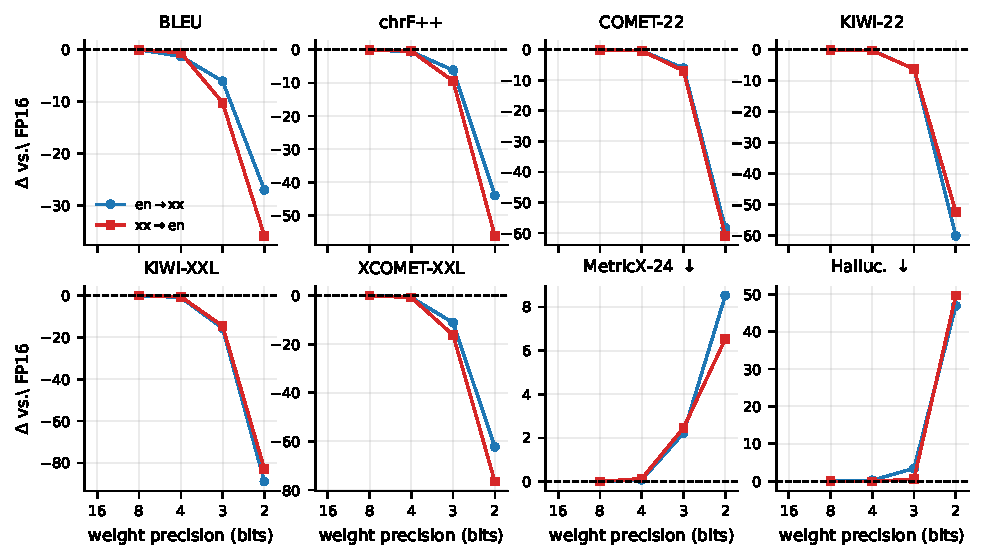
\includegraphics[width=\linewidth]{../figures/fig1_degradation.pdf}
\caption{Every metric against the FP16 beam baseline, per translation direction. The x axis is the weight precision, one tick per quantized checkpoint; the dashed line is FP16 itself, so a point below it (above, for the two marked $\downarrow$) is a loss. A precision whose run has no scores yet is simply absent from the axis.}
\label{fig:fig1_degradation}
\end{figure*}

\begin{figure*}[t]
\centering
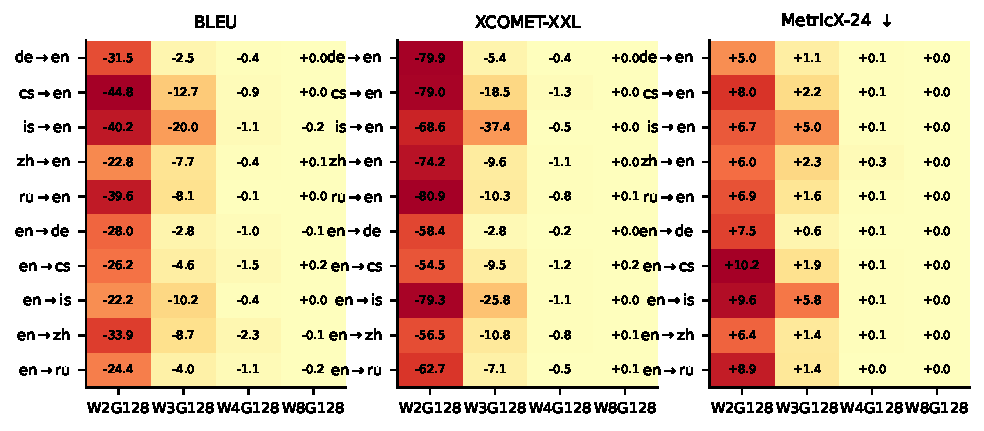
\includegraphics[width=\linewidth]{../figures/fig2_heatmap.pdf}
\caption{Difference against FP16 per direction and precision, coloured so that red is worse and green is better. MetricX-24 is sign-flipped for the colour only: the printed number is the real $\Delta$, and its sign is the opposite of the colour. Each panel is scaled to its own worst cell, so the panels are comparable in shape, not in magnitude.}
\label{fig:fig2_heatmap}
\end{figure*}

\begin{figure*}[t]
\centering
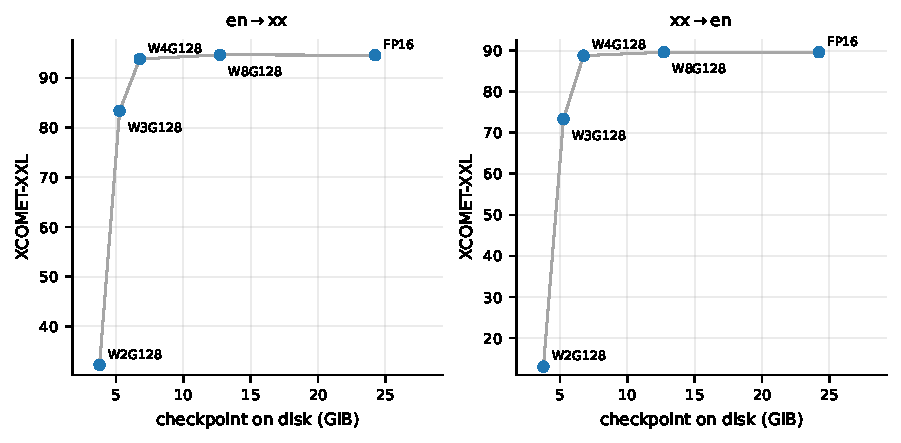
\includegraphics[width=\linewidth]{../figures/fig3_size_quality.pdf}
\caption{XCOMET-XXL against the checkpoint size on disk for both halves of the grid. The 8-bit checkpoint is 1.9$\times$ smaller and indistinguishable from FP16; 4 bits costs well under a point for another 1.9$\times$; the 3-bit step is where both the size and the score move.}
\label{fig:fig3_size_quality}
\end{figure*}

\begin{figure*}[t]
\centering
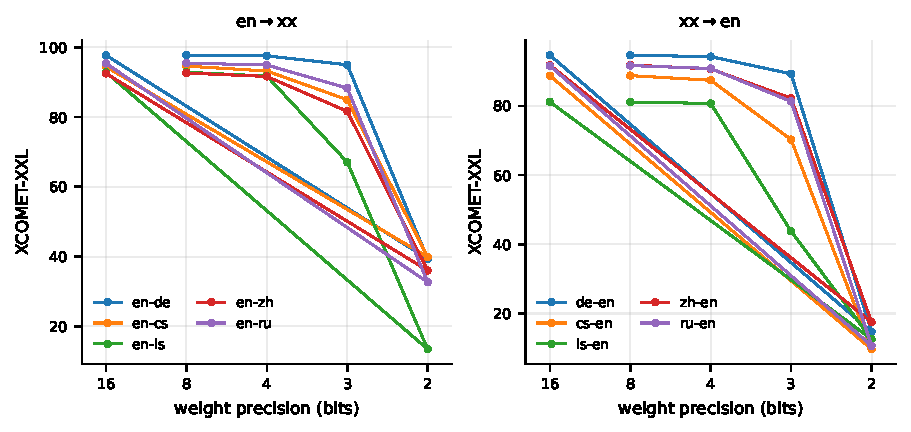
\includegraphics[width=\linewidth]{../figures/fig4_xcometxxl.pdf}
\caption{XCOMET-XXL per direction across the precision grid. All ten directions are hit, but not evenly: the low-resource ones (\texttt{is}, \texttt{zh}, \texttt{cs}) lose several times what \texttt{de} or \texttt{ru} lose at the same precision.}
\label{fig:fig4_xcometxxl}
\end{figure*}

\begin{figure*}[t]
\centering
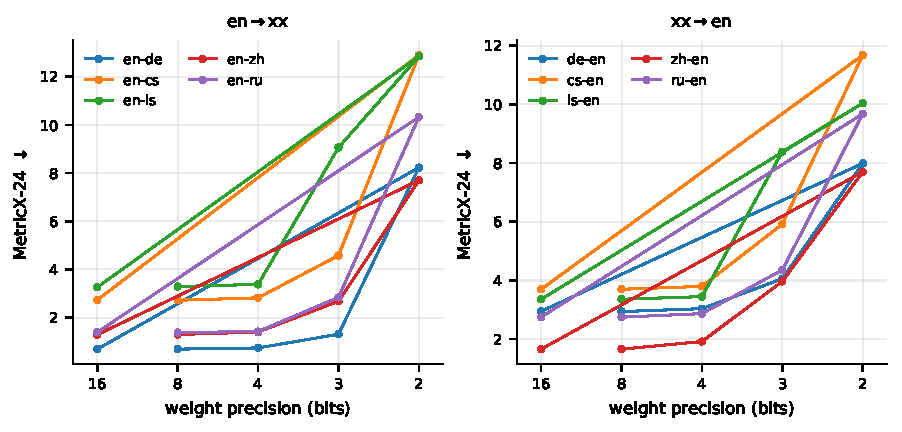
\includegraphics[width=\linewidth]{../figures/fig4_metricx24.pdf}
\caption{MetricX-24 per direction across the precision grid. All ten directions are hit, but not evenly: the low-resource ones (\texttt{is}, \texttt{zh}, \texttt{cs}) lose several times what \texttt{de} or \texttt{ru} lose at the same precision.}
\label{fig:fig4_metricx24}
\end{figure*}

\begin{figure*}[t]
\centering
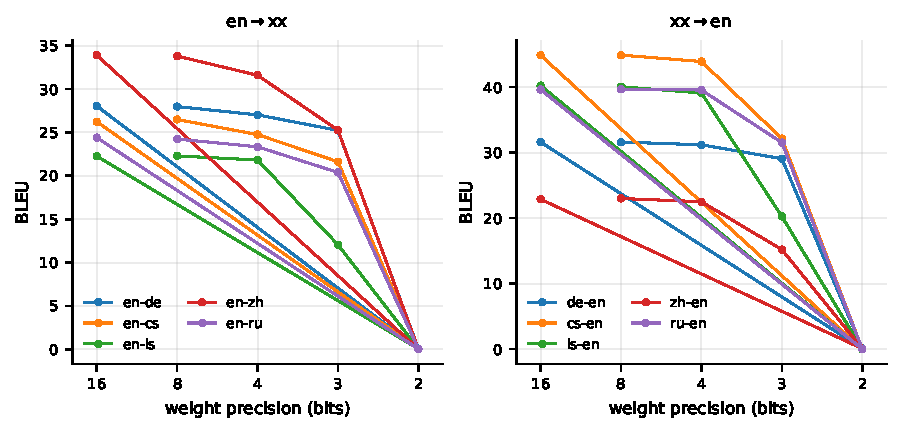
\includegraphics[width=\linewidth]{../figures/fig4_bleu.pdf}
\caption{BLEU per direction across the precision grid. All ten directions are hit, but not evenly: the low-resource ones (\texttt{is}, \texttt{zh}, \texttt{cs}) lose several times what \texttt{de} or \texttt{ru} lose at the same precision.}
\label{fig:fig4_bleu}
\end{figure*}

\begin{figure*}[t]
\centering
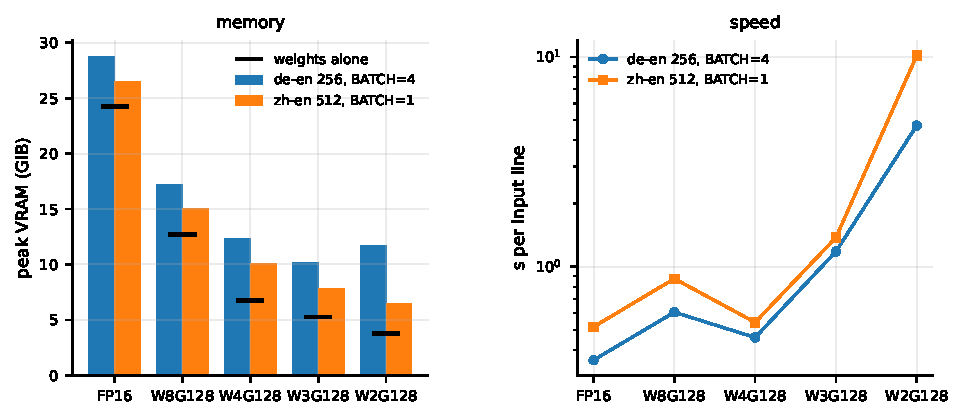
\includegraphics[width=\linewidth]{../figures/fig5_cost.pdf}
\caption{Left: the allocator peak of a timed \texttt{generate()} at the two eval protocols, with the model's own parameter footprint marked. The weights are what the compression shrinks; the rest of the bar is the KV cache and the activations, which no weight-only scheme touches, so the saving saturates well before it reaches the weights' ratio - and w2's peak rises again over w4's, because it generates 180-token outputs where w4 generates 40 and the extra KV cache outweighs the smaller weights. Right: the same checkpoints' cost per input line, log scale. The low-bit checkpoints are not cheaper per line than fp16 on this stack - GPTQModel's Triton/Torch kernels dequantize the weights and then matmul (\texttt{quant\_matmul} in \texttt{triton\_utils/dequant.py}), so every forward pays for weights it never stores - unless the batch is raised (see the batch-size section).}
\label{fig:fig5_cost}
\end{figure*}

\begin{figure*}[t]
\centering
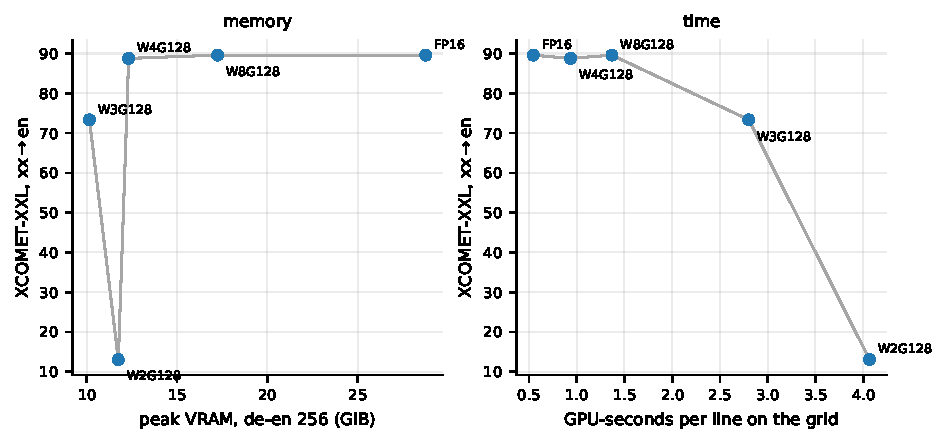
\includegraphics[width=\linewidth]{../figures/fig6_trade.pdf}
\caption{The trade the grid made. XCOMET-XXL is the harness the 3-bit collapse shows up in first (81.15 to 43.75 on \texttt{is-en}), so it is the metric that separates the two checkpoints that are worth keeping from the two that are not. Memory is the de-en \texttt{BATCH=4} peak; time is the measured grid (generation only), GPU-seconds per scored line.}
\label{fig:fig6_trade}
\end{figure*}



\clearpage
\section*{Per-direction numbers}
\begin{table}[t]
\centering
\small
\begin{tabular}{lrrrrrrr}
\toprule
& W2G128 & W3G128 & W4G128 & W8G128 & FP16 & FP16 (sampling) & paper \\
\midrule
de$\rightarrow$en & 0.10 & 29.06 & 31.18 & 31.60 & 31.59 & 31.59 & 30.89 \\
cs$\rightarrow$en & 0.01 & 32.13 & 43.89 & 44.86 & 44.83 & 44.85 & 44.39 \\
is$\rightarrow$en & 0.00 & 20.25 & 39.09 & 40.04 & 40.21 & 40.15 & 39.67 \\
zh$\rightarrow$en & 0.08 & 15.19 & 22.49 & 22.99 & 22.87 & 22.99 & 23.23 \\
ru$\rightarrow$en & 0.02 & 31.52 & 39.54 & 39.64 & 39.61 & 39.65 & 39.06 \\
en$\rightarrow$de & 0.04 & 25.24 & 27.03 & 27.99 & 28.05 & 27.88 & 27.72 \\
en$\rightarrow$cs & 0.06 & 21.62 & 24.76 & 26.50 & 26.25 & 26.16 & 26.32 \\
en$\rightarrow$is & 0.04 & 12.05 & 21.82 & 22.30 & 22.26 & 22.17 & 22.88 \\
en$\rightarrow$zh & 0.01 & 25.27 & 31.60 & 33.81 & 33.92 & 33.89 & 34.06 \\
en$\rightarrow$ru & 0.02 & 20.39 & 23.35 & 24.24 & 24.41 & 24.36 & 24.15 \\
\midrule
avg\_en$\rightarrow$xx & 0.03 & 20.91 & 25.71 & 26.97 & 26.98 & 26.89 & 27.03 \\
avg\_xx$\rightarrow$en & 0.04 & 25.63 & 35.24 & 35.83 & 35.82 & 35.85 & 35.45 \\
\bottomrule
\end{tabular}
\caption{BLEU by direction, with the ALMA-R paper's own reported numbers.}
\label{tab:bleu}
\end{table}

\begin{table}[t]
\centering
\small
\begin{tabular}{lrrrrrr}
\toprule
& W2G128 & W3G128 & W4G128 & W8G128 & FP16 & FP16 (sampling) \\
\midrule
de$\rightarrow$en & 4.71 & 52.80 & 55.03 & 55.27 & 55.27 & 55.25 \\
cs$\rightarrow$en & 3.47 & 56.68 & 66.52 & 67.35 & 67.33 & 67.30 \\
is$\rightarrow$en & 4.37 & 43.15 & 61.13 & 61.69 & 61.72 & 61.65 \\
zh$\rightarrow$en & 3.83 & 42.78 & 51.79 & 52.26 & 52.20 & 52.24 \\
ru$\rightarrow$en & 3.39 & 58.11 & 64.16 & 64.21 & 64.17 & 64.21 \\
en$\rightarrow$de & 6.45 & 52.50 & 54.95 & 55.63 & 55.66 & 55.53 \\
en$\rightarrow$cs & 4.65 & 47.59 & 51.62 & 52.36 & 52.25 & 52.30 \\
en$\rightarrow$is & 5.09 & 38.50 & 50.32 & 50.56 & 50.58 & 50.52 \\
en$\rightarrow$zh & 0.36 & 21.98 & 27.46 & 28.23 & 28.37 & 28.53 \\
en$\rightarrow$ru & 0.51 & 45.54 & 49.72 & 50.01 & 50.08 & 50.13 \\
\midrule
avg\_en$\rightarrow$xx & 3.41 & 41.22 & 46.81 & 47.36 & 47.39 & 47.40 \\
avg\_xx$\rightarrow$en & 3.95 & 50.70 & 59.73 & 60.16 & 60.14 & 60.13 \\
\bottomrule
\end{tabular}
\caption{chrF++ by direction.}
\label{tab:chrf}
\end{table}

\begin{table}[t]
\centering
\small
\begin{tabular}{lrrrrrrr}
\toprule
& W2G128 & W3G128 & W4G128 & W8G128 & FP16 & FP16 (sampling) & paper \\
\midrule
de$\rightarrow$en & 26.51 & 82.32 & 84.76 & 85.02 & 85.02 & 84.99 & 84.95 \\
cs$\rightarrow$en & 23.77 & 80.76 & 86.67 & 87.00 & 87.00 & 86.99 & 86.85 \\
is$\rightarrow$en & 23.63 & 73.08 & 86.83 & 87.25 & 87.26 & 87.24 & 87.14 \\
zh$\rightarrow$en & 24.94 & 75.17 & 81.07 & 81.61 & 81.58 & 81.60 & 81.64 \\
ru$\rightarrow$en & 22.90 & 80.63 & 85.31 & 85.58 & 85.59 & 85.60 & 85.45 \\
en$\rightarrow$de & 34.22 & 84.07 & 86.47 & 86.85 & 86.93 & 86.88 & 86.40 \\
en$\rightarrow$cs & 34.15 & 86.32 & 90.27 & 90.56 & 90.60 & 90.52 & 90.29 \\
en$\rightarrow$is & 20.92 & 74.00 & 86.77 & 87.03 & 87.05 & 87.12 & 86.85 \\
en$\rightarrow$zh & 33.89 & 81.24 & 86.53 & 87.04 & 87.03 & 87.05 & 86.86 \\
en$\rightarrow$ru & 25.51 & 84.46 & 88.50 & 88.73 & 88.75 & 88.78 & 88.30 \\
\midrule
avg\_en$\rightarrow$xx & 29.74 & 82.02 & 87.71 & 88.04 & 88.07 & 88.07 & 87.74 \\
avg\_xx$\rightarrow$en & 24.35 & 78.39 & 84.93 & 85.29 & 85.29 & 85.28 & 85.21 \\
\bottomrule
\end{tabular}
\caption{COMET-22 by direction, with the ALMA-R paper's own reported numbers.}
\label{tab:comet-22}
\end{table}

\begin{table}[t]
\centering
\small
\begin{tabular}{lrrrrrrr}
\toprule
& W2G128 & W3G128 & W4G128 & W8G128 & FP16 & FP16 (sampling) & paper \\
\midrule
de$\rightarrow$en & 28.14 & 79.01 & 81.50 & 81.69 & 81.69 & 81.69 & 81.50 \\
cs$\rightarrow$en & 26.51 & 76.66 & 82.69 & 82.79 & 82.78 & 82.76 & 82.63 \\
is$\rightarrow$en & 34.41 & 70.49 & 81.54 & 81.66 & 81.68 & 81.67 & 81.57 \\
zh$\rightarrow$en & 27.44 & 72.75 & 78.86 & 79.51 & 79.46 & 79.54 & 79.24 \\
ru$\rightarrow$en & 29.29 & 77.46 & 81.60 & 81.90 & 81.89 & 81.88 & 81.72 \\
en$\rightarrow$de & 23.93 & 80.98 & 83.40 & 83.69 & 83.69 & 83.68 & 83.28 \\
en$\rightarrow$cs & 23.83 & 80.41 & 85.17 & 85.34 & 85.37 & 85.40 & 84.99 \\
en$\rightarrow$is & 21.25 & 69.83 & 82.14 & 82.39 & 82.44 & 82.58 & 82.18 \\
en$\rightarrow$zh & 24.61 & 76.35 & 82.31 & 82.59 & 82.58 & 82.61 & 82.25 \\
en$\rightarrow$ru & 24.18 & 79.83 & 84.24 & 84.43 & 84.40 & 84.45 & 83.98 \\
\midrule
avg\_en$\rightarrow$xx & 23.56 & 77.48 & 83.45 & 83.69 & 83.70 & 83.74 & 83.34 \\
avg\_xx$\rightarrow$en & 29.16 & 75.27 & 81.24 & 81.51 & 81.50 & 81.51 & 81.33 \\
\bottomrule
\end{tabular}
\caption{KIWI-22 by direction, with the ALMA-R paper's own reported numbers.}
\label{tab:kiwi-22}
\end{table}

\begin{table}[t]
\centering
\small
\begin{tabular}{lrrrrrrr}
\toprule
& W2G128 & W3G128 & W4G128 & W8G128 & FP16 & FP16 (sampling) & paper \\
\midrule
de$\rightarrow$en & 0.35 & 77.68 & 84.04 & 84.48 & 84.45 & 84.43 & 83.97 \\
cs$\rightarrow$en & -1.38 & 68.33 & 83.56 & 84.26 & 84.22 & 84.18 & 83.75 \\
is$\rightarrow$en & -1.02 & 58.13 & 85.53 & 85.95 & 85.97 & 85.93 & 85.73 \\
zh$\rightarrow$en & 2.24 & 64.31 & 76.49 & 77.51 & 77.37 & 77.50 & 77.17 \\
ru$\rightarrow$en & -0.87 & 72.13 & 81.16 & 81.70 & 81.69 & 81.76 & 81.54 \\
en$\rightarrow$de & -2.09 & 77.76 & 84.46 & 85.31 & 85.30 & 85.25 & 84.25 \\
en$\rightarrow$cs & -1.34 & 75.17 & 87.55 & 88.74 & 88.74 & 88.53 & 87.06 \\
en$\rightarrow$is & -3.68 & 56.31 & 85.58 & 86.30 & 86.41 & 86.58 & 85.68 \\
en$\rightarrow$zh & -1.62 & 70.56 & 84.26 & 85.14 & 85.23 & 85.25 & 84.32 \\
en$\rightarrow$ru & -1.88 & 75.97 & 87.51 & 88.36 & 88.28 & 88.27 & 87.37 \\
\midrule
avg\_en$\rightarrow$xx & -2.12 & 71.15 & 85.87 & 86.77 & 86.79 & 86.78 & 85.74 \\
avg\_xx$\rightarrow$en & -0.14 & 68.12 & 82.16 & 82.78 & 82.74 & 82.76 & 82.43 \\
\bottomrule
\end{tabular}
\caption{KIWI-XXL by direction, with the ALMA-R paper's own reported numbers.}
\label{tab:kiwi-xxl}
\end{table}

\begin{table}[t]
\centering
\small
\begin{tabular}{lrrrrrrr}
\toprule
& W2G128 & W3G128 & W4G128 & W8G128 & FP16 & FP16 (sampling) & paper \\
\midrule
de$\rightarrow$en & 14.72 & 89.25 & 94.24 & 94.63 & 94.66 & 94.67 & 94.20 \\
cs$\rightarrow$en & 9.70 & 70.26 & 87.40 & 88.75 & 88.73 & 88.63 & 88.03 \\
is$\rightarrow$en & 12.60 & 43.75 & 80.70 & 81.12 & 81.15 & 81.12 & 80.49 \\
zh$\rightarrow$en & 17.53 & 82.18 & 90.67 & 91.81 & 91.78 & 91.91 & 91.65 \\
ru$\rightarrow$en & 10.68 & 81.28 & 90.80 & 91.65 & 91.55 & 91.55 & 91.18 \\
en$\rightarrow$de & 39.32 & 94.96 & 97.53 & 97.73 & 97.71 & 97.70 & 97.48 \\
en$\rightarrow$cs & 39.88 & 84.94 & 93.18 & 94.59 & 94.41 & 94.42 & 93.61 \\
en$\rightarrow$is & 13.47 & 67.05 & 91.73 & 92.82 & 92.82 & 93.27 & 91.93 \\
en$\rightarrow$zh & 36.01 & 81.63 & 91.62 & 92.61 & 92.47 & 92.61 & 92.03 \\
en$\rightarrow$ru & 32.65 & 88.27 & 94.90 & 95.45 & 95.36 & 95.37 & 95.22 \\
\midrule
avg\_en$\rightarrow$xx & 32.27 & 83.37 & 93.79 & 94.64 & 94.55 & 94.67 & 94.05 \\
avg\_xx$\rightarrow$en & 13.05 & 73.34 & 88.76 & 89.59 & 89.57 & 89.58 & 89.11 \\
\bottomrule
\end{tabular}
\caption{XCOMET-XXL by direction, with the ALMA-R paper's own reported numbers.}
\label{tab:xcomet-xxl}
\end{table}

\begin{table}[t]
\centering
\small
\begin{tabular}{lrrrrrr}
\toprule
& W2G128 & W3G128 & W4G128 & W8G128 & FP16 & FP16 (sampling) \\
\midrule
de$\rightarrow$en & 7.99 & 4.06 & 3.04 & 2.94 & 2.95 & 2.95 \\
cs$\rightarrow$en & 11.68 & 5.92 & 3.80 & 3.70 & 3.70 & 3.70 \\
is$\rightarrow$en & 10.04 & 8.39 & 3.45 & 3.36 & 3.36 & 3.36 \\
zh$\rightarrow$en & 7.70 & 3.97 & 1.92 & 1.66 & 1.66 & 1.65 \\
ru$\rightarrow$en & 9.68 & 4.36 & 2.87 & 2.75 & 2.75 & 2.75 \\
en$\rightarrow$de & 8.23 & 1.31 & 0.74 & 0.69 & 0.69 & 0.68 \\
en$\rightarrow$cs & 12.90 & 4.58 & 2.82 & 2.72 & 2.73 & 2.72 \\
en$\rightarrow$is & 12.85 & 9.06 & 3.38 & 3.29 & 3.26 & 3.24 \\
en$\rightarrow$zh & 7.70 & 2.68 & 1.40 & 1.30 & 1.29 & 1.30 \\
en$\rightarrow$ru & 10.33 & 2.84 & 1.42 & 1.38 & 1.39 & 1.40 \\
\midrule
avg\_en$\rightarrow$xx & 10.40 & 4.09 & 1.95 & 1.88 & 1.87 & 1.87 \\
avg\_xx$\rightarrow$en & 9.42 & 5.34 & 3.02 & 2.88 & 2.88 & 2.88 \\
\bottomrule
\end{tabular}
\caption{MetricX-24 by direction.}
\label{tab:metricx-24}
\end{table}

\begin{table}[t]
\centering
\small
\begin{tabular}{lrrrrrr}
\toprule
& W2G128 & W3G128 & W4G128 & W8G128 & FP16 & FP16 (sampling) \\
\midrule
de$\rightarrow$en & 62.05 & 0.10 & 0.00 & 0.05 & 0.05 & 0.05 \\
cs$\rightarrow$en & 46.27 & 0.21 & 0.00 & 0.07 & 0.07 & 0.07 \\
is$\rightarrow$en & 42.70 & 0.80 & 0.00 & 0.00 & 0.00 & 0.00 \\
zh$\rightarrow$en & 40.80 & 2.29 & 0.37 & 0.59 & 0.53 & 0.48 \\
ru$\rightarrow$en & 57.34 & 0.30 & 0.00 & 0.10 & 0.15 & 0.15 \\
en$\rightarrow$de & 42.46 & 0.25 & 0.20 & 0.20 & 0.20 & 0.20 \\
en$\rightarrow$cs & 31.81 & 2.31 & 0.44 & 0.39 & 0.49 & 0.49 \\
en$\rightarrow$is & 39.40 & 9.90 & 0.10 & 0.20 & 0.20 & 0.00 \\
en$\rightarrow$zh & 93.13 & 5.06 & 2.65 & 1.82 & 1.72 & 1.72 \\
en$\rightarrow$ru & 30.34 & 2.55 & 0.64 & 0.29 & 0.25 & 0.29 \\
\midrule
avg\_en$\rightarrow$xx & 47.43 & 4.01 & 0.81 & 0.58 & 0.57 & 0.54 \\
avg\_xx$\rightarrow$en & 49.83 & 0.74 & 0.07 & 0.16 & 0.16 & 0.15 \\
\bottomrule
\end{tabular}
\caption{Halluc. by direction.}
\label{tab:halluc}
\end{table}



\end{document}
